Vorweg will ich kurz erklären, was es mit den Tools zur Versionskontrolle auf sich hat.\\
\ \\
Es geht immer darum, eine lokale Kopie der Quellen von einem Server zu laden. Im einfachsten Fall bei Github als ZIP-Datei. Dies ist in den meisten Fälle ausreichend. Der Link ist jedoch für unsere Versionskontrolle interessant. Dort liegt nun das Repository die ich nenne sie jetzt mal Masterkopie. \\
\begin{minipage}[t]{\textwidth}
  \centering
  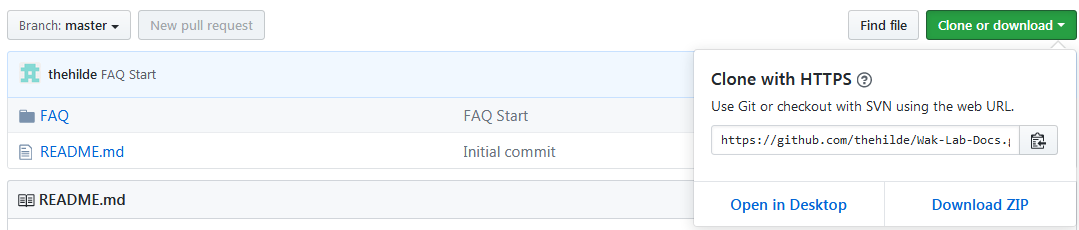
\includegraphics[width=\textwidth]{pictures/Clone.png}
  \captionof{figure}{Eine lokale Kopie Clonen}
  \label{img:Clone}
\end{minipage}
\ \\
Spannend wird es jedoch, wenn die Quellen sich auf dem Server weiterentwickeln oder man sogar selbst eine Verbesserung einbringen will. Die Tools GIT oder SVN managen nun die Synchronisation mit dem Server. Es kann der zeitliche Verlauf der Änderungen angezeigt und zu beliebigen Punkten zurück gesprungen werden. Nie wieder ein "Gestern ging es noch bevor das umgestrickt habe <aarg!>". Welche Änderungen habe ich vor 3 Jahren für XY rein gehackt? Und vor allem Warum? Welchen Fehler wollte ich beseitigen, welches Ticket habe ich bearbeitet? Oder war es der Kollege?  \\
Tools wie Tortoise SVN besitzen eine Explorer Integration, arbeiten über das Kontextmenü und zeigen alle Änderungen automatisch an. \\
\begin{minipage}[t]{\textwidth}
  \centering
  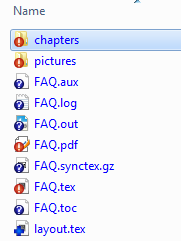
\includegraphics[height=3cm]{pictures/TortoiseSVNChanges.png}
  \captionof{figure}{Tortoise SVN Explorer Integration}
  \label{img:TortoiseSVNChanges}
\end{minipage}
\ \\
Finden Änderungen in der selben Datei aber in unterschiedlichen Bereichen statt, kann das Tool die Änderungen automatisch zusammenführen. In manchen Fällen muss dies jedoch händisch erfolgen.\\
\ \\
Es soll noch gesagt sein, das GIT und SVN zwei verschiedene Tools sind, die etwas abweichende Philosophien haben. Zum Glück sind die beiden auf Github gut verheiratet worden.\\
\ \\
Folgende Dateitypen sind Textbasiert und können prima verwaltet werden.
\begin{itemize}
\item Arduino .ino Dateien
\item Quelltexte z.B. .c .cpp .h .pas .vhdl
\item Natürlich .html .php
\item Windows .ini Dateien
\item Eagle Layout Dateien und Bibliotheken ab Version 6
\item STM Cube32 Dateien
\item \LaTeX .tex Dateien
\item Auch Word ist Prima integriert in Tortoise SVN und öffnet den Word eigenen DIF Viewer.
\end{itemize}


  





